\chapter{मूल कोशिकाएँ, पुनर्जनन और वृद्धावस्था}\label{ch:b3:stem-cells}

किसी ऐक्सोलोटल की टाँग काट दीजिए और दो महीनों में उसने नई उगा ली है,
जिसमें अस्थि, पेशी, तंत्रिका और त्वचा सही जगहों पर हैं, और वह ऐसा उतनी
ही बार करेगा जितनी बार आप काटें। किसी प्लेनेरिया चपटे कृमि को बीस
टुकड़ों में काटिए और हर एक पखवाड़े भर में पूरा कृमि बन जाता है, और जो
टुकड़ा पूँछ था वह आँखों तथा मस्तिष्क वाला कोई सिर फिर उगा लेता है। किसी
मनुष्य की उँगली आख़िरी जोड़ के ऊपर से काट दीजिए और वह किसी व्रणचिह्न के
रूप में भर जाती है। फिर भी मानव शरीर नवीकरण से रहित नहीं: वह हर सेकंड
बीस लाख लाल रक्त-कोशिकाएँ बनाता है, आँत का अस्तर हर पाँच दिन में बदल
जाता है, त्वचा हर महीने, और यह सब कोशिकाओं की उन छोटी समष्टियों से उतरता
है जो जीवन भर बँटती रहती हैं और फिर भी चुकतीं नहीं। यह अध्याय उन्हीं
कोशिकाओं के बारे में है --- कोई \omterm{def:b3:stem-cells:stem}{मूल कोशिका} बनती किससे है, उसका \omterm{def:b3:stem-cells:stem}{कोटर} उसे
कैसे थामे रखता है, रक्त या आँत की पूरी पदानुक्रमी उससे कैसे बनती है ---
उन प्राणियों के बारे में जो वह फिर उगा लेते हैं जो हम नहीं उगा सकते और
क्यों, इस खोज के बारे में कि कोई भी कोशिका चार जीनों से भ्रूणीय अवस्था
तक वापस धकेली जा सकती है, और इस बारे में कि कोशिका-विभाजन का अंकगणित
हमारे बूढ़े होने के बारे में क्या कहता है।

\section{मूल कोशिका है क्या}

\begin{definition}[मूल कोशिकाएँ और उनकी पदानुक्रमी]\label{def:b3:stem-cells:stem}
\index{मूल कोशिका}\index{स्व-नवीकरण}\index{असममित विभाजन}\index{पूर्वगामी}\index{संक्रमण-प्रवर्धी कोशिका}\index{कोटर}
किसी \emph{मूल कोशिका} के दो परिभाषक गुण हैं: वह \emph{स्व-नवीकरण} कर
सकती है, यानी ऐसी संततियाँ बना सकती है जो मूल कोशिकाएँ हों, और वह ऐसी
संततियाँ भी बना सकती है जो विभेदित हों। वह दोनों एक साथ कर सकती है,
\emph{असममित विभाजन} से, यानी हर तरह की एक-एक संतति, जिनका भवितव्य
निर्धारकों की असमान वंशागति से या इससे तय होता है कि कौन-सी संतति उस
\emph{कोटर} के संपर्क में रहती है --- यानी पड़ोसी कोशिकाओं, आधात्री तथा
संकेतों के उस सूक्ष्म-परिवेश के, जो किसी कोशिका को मूल कोशिका बनाए रखता
है; या वह सममित रूप से भी बँट सकती है, जिसमें कुछ विभाजन दो मूल
कोशिकाएँ देते हैं और दूसरे दो विभेदित होती कोशिकाएँ, और वह समष्टि औसतन
अचर बनी रहती है। विभेदित होती संततियाँ प्रायः \emph{पूर्वगामी} या
\emph{संक्रमण-प्रवर्धी} चरणों से गुज़रती हैं, और परिपक्व होने से पहले
सँकरी होती शक्ति के साथ कई बार और बँटती हैं: वह पदानुक्रमी कुछ ही धीमे
मूल-कोशिका विभाजनों को किसी बड़े निर्गम में प्रवर्धित कर देती है, और
किसी भी मूल कोशिका के ज़रूरी विभाजनों की संख्या सीमित कर देती है। वयस्क
मूल कोशिकाएँ दुर्लभ और धीमी होती हैं --- कोई रुधिरजनक मूल कोशिका शायद
साल में एक बार बँटती है, कोई आंत्र मूल कोशिका दिन में एक बार --- और
\emph{बहुशक्त}, यानी अपने ऊतक की वंश-परंपराओं तक सीमित; और कोरकपुटी के
भीतरी कोशिका-पिंड से आती \omterm{def:b3:stem-cells:pluripotency}{भ्रूणीय मूल कोशिकाएँ} \emph{सर्वशक्त} हैं, जो
शरीर का हर ऊतक बना सकती हैं पर अपरा नहीं।
\end{definition}

\begin{omfigure}
\begin{tikzpicture}[every node/.style={font=\scriptsize}, >=stealth]
  \node[draw, very thick, rounded corners, fill=omDef!25, align=center] (hsc) at (0,3.6) {रुधिरजनक मूल कोशिका\\किसी मनुष्य में $\sim$\num{10000}; $\sim$ साल में एक बार बँटती है};
  \node[draw, thick, rounded corners, fill=omDef!12, align=center] (mpp) at (0,2.4) {बहुशक्त पूर्वगामी};
  \node[draw, thick, rounded corners, fill=omThm!15, align=center] (cmp) at (-3.2,1.2) {मायलॉयड पूर्वगामी};
  \node[draw, thick, rounded corners, fill=omProp!20, align=center] (clp) at (3.2,1.2) {लसीकाभ पूर्वगामी};
  \node[align=center, font=\tiny] (e) at (-5.4,-0.4) {लोहिताणु\\$2\times 10^{11}$/दिन};
  \node[align=center, font=\tiny] (pl) at (-3.6,-0.4) {बिंबाणु\\(महाकेंद्रकाणु)};
  \node[align=center, font=\tiny] (g) at (-1.8,-0.4) {कणिकाणु\\$10^{11}$/दिन};
  \node[align=center, font=\tiny] (m) at (-0.2,-0.4) {एककेंद्रकाणु,\\महाभक्षक};
  \node[align=center, font=\tiny] (b) at (1.8,-0.4) {B कोशिकाएँ};
  \node[align=center, font=\tiny] (t) at (3.4,-0.4) {T कोशिकाएँ};
  \node[align=center, font=\tiny] (nk) at (5.0,-0.4) {NK कोशिकाएँ};
  \draw[->, thick] (hsc) -- (mpp); \draw[->, thick] (mpp) -- (cmp); \draw[->, thick] (mpp) -- (clp);
  \foreach \x in {e,pl,g,m} { \draw[->, thick] (cmp) -- (\x); }
  \foreach \x in {b,t,nk} { \draw[->, thick] (clp) -- (\x); }
  \draw[->, thick, omDef!70!black] (hsc.west) .. controls (-3.0,4.4) and (-3.0,3.0) .. (hsc.south west) node[pos=0.5, left, font=\tiny, omDef!70!black, align=right] {स्व-नवीकरण};
  \node[right, align=left, font=\tiny] at (4.4,3.6) {हर तह अधिक बार बँटती है\\और उसकी शक्ति सँकरी होती है;\\मूल कोशिका से लाल कोशिका तक\\$\sim 20$ विभाजन, इसलिए किसी मूल कोशिका का\\एक विभाजन $\sim 10^{6}$ कोशिकाएँ देता है};
\end{tikzpicture}

{\small रुधिरजनक पदानुक्रमी। मज्जा में कुछ हज़ार धीमी \omterm{def:b3:stem-cells:stem}{मूल कोशिकाएँ} उन
\omterm{def:b3:stem-cells:stem}{पूर्वगामियों} को खिलाती हैं जो तेज़ बँटते और उत्तरोत्तर प्रतिबद्ध होते
हैं, इसलिए दिन भर में खरब भर कोशिकाओं का निर्गम उन \omterm{def:b3:stem-cells:stem}{मूल कोशिकाओं} को लगभग
कुछ भी नहीं पड़ता।}
\end{omfigure}

\begin{proof}[प्रमाण-सामग्री]
टिल और मक्कलॉक (1961) ने घातक रूप से विकिरणित चूहों में मज्जा-कोशिकाएँ
अंतःक्षिप्त कीं और दस दिन बाद प्लीहा पर उभरी गाँठें गिनीं: हर एक कई
वंश-परंपराओं की रक्त-कोशिकाओं की कोई बस्ती थी, जिनकी संख्या अंतःक्षिप्त
कोशिकाओं के समानुपाती थी, और दाता कोशिकाओं के गुणसूत्र चिह्नित करने से
हर बस्ती कोई क्लोन निकली --- यानी किसी एक ही कोशिका ने लाल कोशिकाएँ,
कणिकाणु तथा बिंबाणु बनाए थे, और कुछ बस्तियों में ऐसी कोशिकाएँ थीं जो
किसी दूसरे चूहे में नई बस्तियाँ बो सकती थीं: यानी किसी एक ही कोशिका में
\omterm{def:b3:stem-cells:stem}{स्व-नवीकरण} तथा बहुशक्तता, जो \omterm{def:b3:stem-cells:stem}{मूल कोशिका} की प्रचालनात्मक परिभाषा है और
अस्थि-मज्जा प्रत्यारोपण का आधार। बार्कर और क्लेवर्स (2007) ने आंत्र
क्रिप्टों के आधार पर जीन \emph{Lgr5} अभिव्यक्त करती कोशिकाओं को किसी
वंशागत रंग से चिह्नित किया और हफ़्तों तक देखा कि वह रंग उस क्रिप्ट पर
चढ़कर पूरे रसांकुर भर देता है: वे चिह्नित कोशिकाएँ आँत की \omterm{def:b3:stem-cells:stem}{मूल कोशिकाएँ}
थीं, और उनमें से एक, सही तीन वृद्धि कारकों के साथ किसी जेल में संवर्धित,
अपने ही क्रिप्टों तथा रसांकुरों वाली कोई नन्ही आँत, यानी कोई
\emph{\omterm{def:b3:stem-cells:pluripotency}{ऑर्गेनॉइड}}, बन गई (सातो, 2009)।
\end{proof}

\begin{proposition}[कोटर और क्रिप्ट]\label{prop:b3:stem-cells:crypt}
\index{क्रिप्ट}\index{Lgr5}\index{पैनेथ कोशिका}\index{Wnt संकेतन}\index{उदासीन अपवाह}
आंत्र \emph{क्रिप्ट} सबसे अच्छी तरह समझा गया \omterm{def:b3:stem-cells:stem}{कोटर} है। उसके आधार पर
लगभग चौदह \emph{Lgr5} \omterm{def:b3:stem-cells:stem}{मूल कोशिकाएँ} \omterm{prop:b3:stem-cells:crypt}{पैनेथ कोशिकाओं} के बीच ठुँसी बैठी
हैं, जो वे Wnt तथा Notch संकेत और वृद्धि कारक स्रवित करती हैं जो उन्हें
\omterm{def:b3:stem-cells:stem}{मूल कोशिकाएँ} बनाए रखते हैं; और जो \omterm{def:b3:stem-cells:stem}{मूल कोशिका} ऊपर धकेलकर \omterm{prop:b3:stem-cells:crypt}{पैनेथ कोशिकाओं}
के संपर्क से बाहर हो जाए वह कुछ ही कोशिका-व्यासों में वह संकेत खो देती
है और कोई \omterm{def:b3:stem-cells:stem}{संक्रमण-प्रवर्धी कोशिका} बन जाती है, जो उस क्रिप्ट में चार-पाँच
बार बँटती है और फिर उन अवशोषी तथा स्रावी कोशिकाओं में विभेदित होती है जो
रसांकुर पर ऊपर चढ़ती हैं और पाँच दिन बाद उसकी नोक से झड़ जाती हैं। वे
\omterm{def:b3:stem-cells:stem}{मूल कोशिकाएँ} सममित रूप से, लगभग दिन में एक बार, बँटती हैं और उस सीमित
कोटर-स्थान के लिए स्पर्धा करती हैं: संयोग से कोई एक क्लोन फैलता है और
बाकी खो जाते हैं, इसलिए कुछ ही महीनों में हर क्रिप्ट किसी एक ही \omterm{def:b3:stem-cells:stem}{मूल
कोशिका} से उतरा होता है --- यानी क्रिप्ट के पैमाने पर \emph{\omterm{prop:b3:stem-cells:crypt}{उदासीन
अपवाह}}, यानी अवशोषी सीमाओं वाला कोई यादृच्छिक चलन। वह \omterm{def:b3:stem-cells:stem}{कोटर}, न कि वह
कोशिका, उस मूलत्व को थामे है: चोट के बाद किसी विभेदित कोशिका को पैनेथ
संकेतों के संपर्क में वापस रखिए और वह पलट सकती है; उस \omterm{def:b3:stem-cells:stem}{मूल कोशिका} को
बाहर निकालकर किसी तश्तरी में वे संकेत दीजिए और वह कोई \omterm{def:b3:stem-cells:pluripotency}{ऑर्गेनॉइड} बना
देती है। अस्थि-मज्जा, रोम-पुटक, वृषण और मस्तिष्क के तंत्रिकीय मूल-कोशिका
क्षेत्र भिन्न संकेतों के साथ उसी तर्क पर चलते हैं।
\end{proposition}
\begin{proof}[प्रमाण-सामग्री]
स्निपर्ट और सहयोगियों (2010) ने क्रिप्ट की \omterm{def:b3:stem-cells:stem}{मूल कोशिकाएँ} चार यादृच्छिक
रंगों की किसी ``कन्फ़ेटी'' से चिह्नित कीं; वे क्रिप्ट पहले बहुरंगी थे और
कुछ महीनों में एकरंगी हो गए, और वह दर सममित विभाजन तथा लगभग चौदह
कोशिकाओं के बीच उदासीन स्पर्धा से मेल खाती थी --- न कि \omterm{def:b3:stem-cells:stem}{असममित विभाजन}
से, जो हर रंग को अनिश्चित काल तक बनाए रखता। \omterm{prop:b3:stem-cells:crypt}{पैनेथ कोशिकाएँ} हटाने से वह
मूल-कोशिका पूल सिकुड़ जाता है; और Wnt संकेत हटाने से वह क्रिप्ट दिनों
में ख़ाली हो जाता है।
\end{proof}

\begin{omfigure}
\begin{tikzpicture}[every node/.style={font=\scriptsize}, >=stealth]
  % crypt-villus
  \draw[very thick, omDef] (0,-2.6) .. controls (0,-0.4) and (0.4,0) .. (0.8,0) -- (0.8,3.6) .. controls (0.8,4.1) and (1.6,4.1) .. (1.6,3.6) -- (1.6,0) .. controls (2.0,0) and (2.4,-0.4) .. (2.4,-2.6);
  \draw[very thick, omDef] (0,-2.6) arc[start angle=180, end angle=360, radius=1.2];
  % stem cells at base
  \foreach \a in {200,230,260,290,320} { \fill[omThm!60] ({1.2+1.05*cos(\a)},{-2.6+1.05*sin(\a)}) circle (0.14); }
  \foreach \a in {215,245,275,305} { \fill[omMeth!60] ({1.2+0.75*cos(\a)},{-2.6+0.75*sin(\a)}) circle (0.13); }
  \node[right, align=left, font=\tiny] at (2.6,-3.4) {आधार: $\sim 14$ \emph{Lgr5} मूल कोशिकाएँ (लाल)\\पैनेथ कोशिकाओं (हरी) के बीच ठुँसी,\\जो Wnt, Notch, EGF जुटाती हैं};
  % TA zone
  \foreach \y in {-1.8,-1.3,-0.8,-0.3} { \fill[omProp!50] (0.35,\y) circle (0.11); \fill[omProp!50] (2.05,\y) circle (0.11); }
  \node[right, align=left, font=\tiny] at (2.6,-1.1) {संक्रमण-प्रवर्धी क्षेत्र:\\4--5 विभाजन, दिन में एक,\\पैनेथ संकेतों से परे};
  % villus cells
  \foreach \y in {0.4,1.0,1.6,2.2,2.8} { \fill[omDef!40] (0.95,\y) circle (0.1); \fill[omDef!40] (1.45,\y) circle (0.1); }
  \node[right, align=left, font=\tiny] at (2.6,1.8) {रसांकुर: विभेदित कोशिकाएँ\\ऊपर चढ़ती हैं और $\sim 5$ दिन बाद\\नोक से झड़ जाती हैं};
  \node[left, font=\tiny] at (-0.1,-2.6) {क्रिप्ट}; \node[left, font=\tiny] at (0.7,3.9) {रसांकुर की नोक};
  % confetti panel
  \begin{scope}[shift={(8.8,0.2)}]
    \node[above, align=center] at (0,1.3) {कोटर में उदासीन अपवाह};
    \foreach \i/\cols in {0/{omDef!60,omThm!60,omMeth!60,omProp!60,omDef!60,omThm!60}, 1/{omDef!60,omDef!60,omThm!60,omThm!60,omThm!60,omProp!60}, 2/{omThm!60,omThm!60,omThm!60,omThm!60,omDef!60,omThm!60}, 3/{omThm!60,omThm!60,omThm!60,omThm!60,omThm!60,omThm!60}} {
      \foreach [count=\j] \c in \cols { \fill[\c] ({\j*0.36-1.26},{1.0-\i*0.7}) circle (0.15); }
    }
    \node[left, font=\tiny] at (-1.35,1.0) {सप्ताह 0}; \node[left, font=\tiny] at (-1.35,0.3) {सप्ताह 4}; \node[left, font=\tiny] at (-1.35,-0.4) {सप्ताह 12}; \node[left, font=\tiny] at (-1.35,-1.1) {महीने};
    \node[below, align=center, font=\tiny] at (0,-1.75) {क्लोन जगहों की किसी नियत संख्या के\\लिए स्पर्धा करते हैं; कोई एक संयोग से जीतता है};
  \end{scope}
\end{tikzpicture}

{\small \omterm{def:b3:stem-cells:stem}{कोटर} के रूप में क्रिप्ट। मूलत्व कोई जगह है: जो कोशिकाएँ \omterm{prop:b3:stem-cells:crypt}{पैनेथ
कोशिकाओं} के संकेतों के संपर्क में हैं वे \omterm{def:b3:stem-cells:stem}{मूल कोशिकाएँ} बनी रहती हैं, और
जो संपर्क से बाहर धकेल दी जाती हैं वे रसांकुर की नोक तक की पाँच दिन की
यात्रा शुरू कर देती हैं। यादृच्छिक रंगों से चिह्नित करने पर किसी
क्रिप्ट की \omterm{def:b3:stem-cells:stem}{मूल कोशिकाएँ} महीनों में बहकर किसी एक क्लोन पर आ जाती हैं।}
\end{omfigure}

\section{सर्वशक्तता और पुनःक्रमण}

\begin{definition}[भ्रूणीय, प्रेरित, और संवर्धित]\label{def:b3:stem-cells:pluripotency}
\index{भ्रूणीय मूल कोशिका}\index{सर्वशक्तता}\index{प्रेरित सर्वशक्त मूल कोशिका}\index{पुनःक्रमण}\index{ऑर्गेनॉइड}
\emph{भ्रूणीय \omterm{def:b3:stem-cells:stem}{मूल कोशिकाएँ}} (इवांस, कॉफ़मैन, मार्टिन, 1981, चूहा;
थॉमसन, 1998, मानव) भीतरी कोशिका-पिंड की वे कोशिकाएँ हैं जिन्हें संवर्ध
में बिना विभेदित हुए बँटता रखा जाता है, उन संकेतों से (LIF, या FGF तथा
ऐक्टिविन) जो अनुलेखन कारकों का कोई केंद्रक बनाए रखते हैं --- Oct4,
Sox2, Nanog --- जो एक-दूसरे को सक्रिय करते हैं और हर वंश-परंपरा के जीन
दबाते हैं। किसी कोरकपुटी में अंतःक्षिप्त करने पर वे उस भ्रूण में शामिल
हो जाती हैं और उसके सारे ऊतकों में योग देती हैं, जनन-वंश समेत, और इसी
से नॉकआउट चूहा बनाया जाता है: उन कोशिकाओं में कोई जीन बदलिए, और उनसे कोई
चूहा बना लीजिए। वर्ष~2 के खंड के केंद्रक-अंतरण ने दिखाया था कि किसी
विभेदित केंद्रक को अंडे का कोशिकाद्रव्य फिर से तैयार कर सकता है; और
ताकाहाशी तथा यामानाका (2006) ने पाया कि वह तैयारी करता कौन है। चौबीस
उम्मीदवार जीनों में से चार --- \emph{Oct4}, \emph{Sox2}, \emph{Klf4},
\emph{c-Myc} --- \omterm{def:b3:virology:virus}{विषाणुओं} पर साथ मिलाकर त्वचा के तंतुकोरकों में डाले
जाने पर तीन हफ़्तों में हज़ार में लगभग एक कोशिका को किसी
\emph{प्रेरित सर्वशक्त \omterm{def:b3:stem-cells:stem}{मूल कोशिका}} में बदल देते थे, जो किसी भ्रूणीय
कोशिका से अभेद्य थी और हर ऊतक तथा पूरा चूहा बना सकती थी।
\emph{पुनःक्रमण} धीमा और अकुशल है क्योंकि उन कारकों को वह \omterm{def:b3:chromatin-epigenetics:nucleosome}{क्रोमैटिन}
खोलना पड़ता है जिसे वर्षों के विभेदन ने बंद किया है, और वे कोशिकाएँ
किसी प्रसंभाव्य प्रावस्था से गुज़रती हैं जिसमें अधिकांश अटक जाती हैं;
और वह, सिद्धांततः, किसी रोगी की अपनी कोशिकाओं से किसी भी ऊतक तक का कोई
रास्ता भी है। सही संकेत सही क्रम में जोड़िए और तश्तरी में सर्वशक्त
कोशिकाएँ परिवर्धन दुहरा देती हैं: धड़कती हृद्-पेशी, किसी पार्किंसनी
मस्तिष्क में प्रत्यारोपण के लिए डोपामीन न्यूरॉन, दृष्टिपटलीय कोशिकाएँ,
और \emph{ऑर्गेनॉइड} --- यानी कुछ मिलीमीटर भर के स्वयं-संगठित
त्रि-आयामी ऊतक, आँत, गुर्दा, यकृत तथा प्रमस्तिष्कीय, जिनमें उस अंग की
वास्तु तथा कोशिका-प्रकार हैं, और जिनमें मानव परिवर्धन तथा रोग देखे जा
सकते हैं और औषधें आज़माई जा सकती हैं।
\end{definition}

\begin{omfigure}
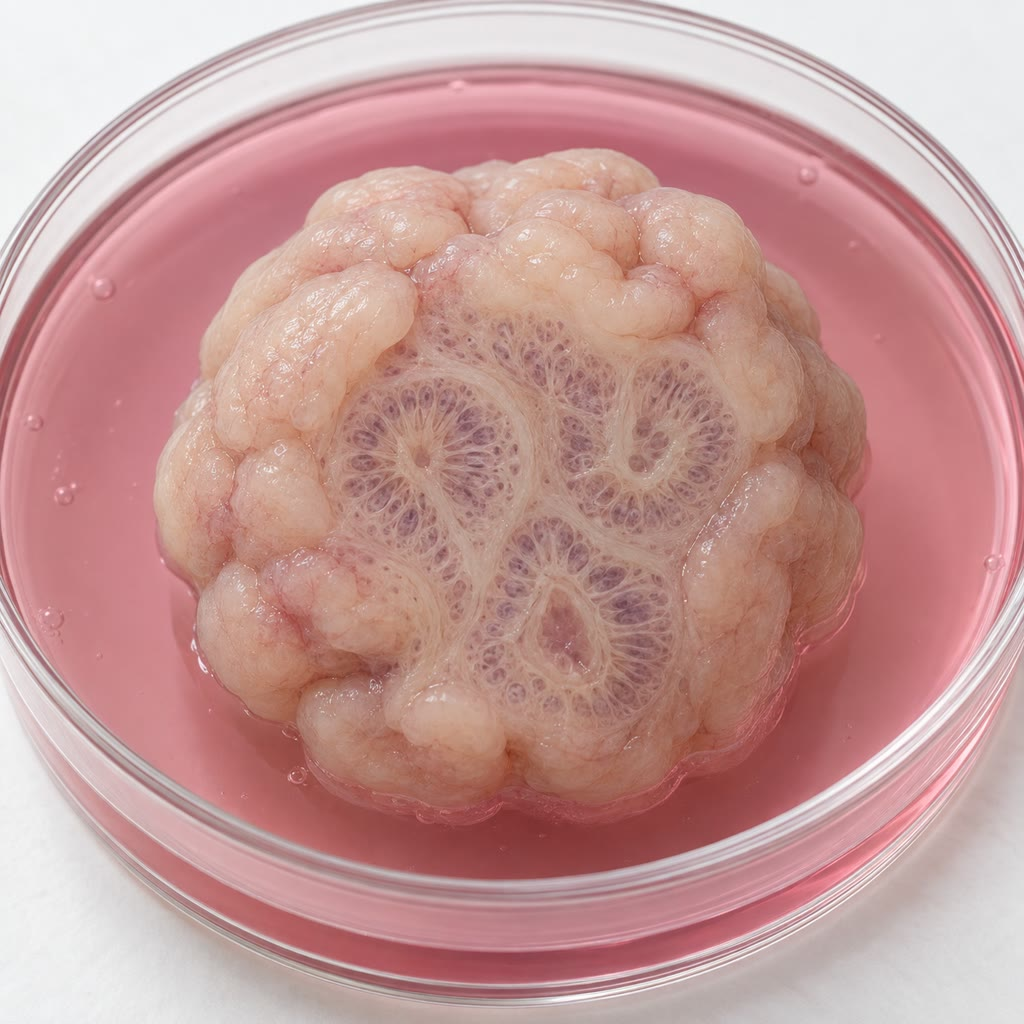
\includegraphics[width=0.4\linewidth]{images/book5/ai/b5-24-brain-organoid.jpg}\hspace{0.04\linewidth}
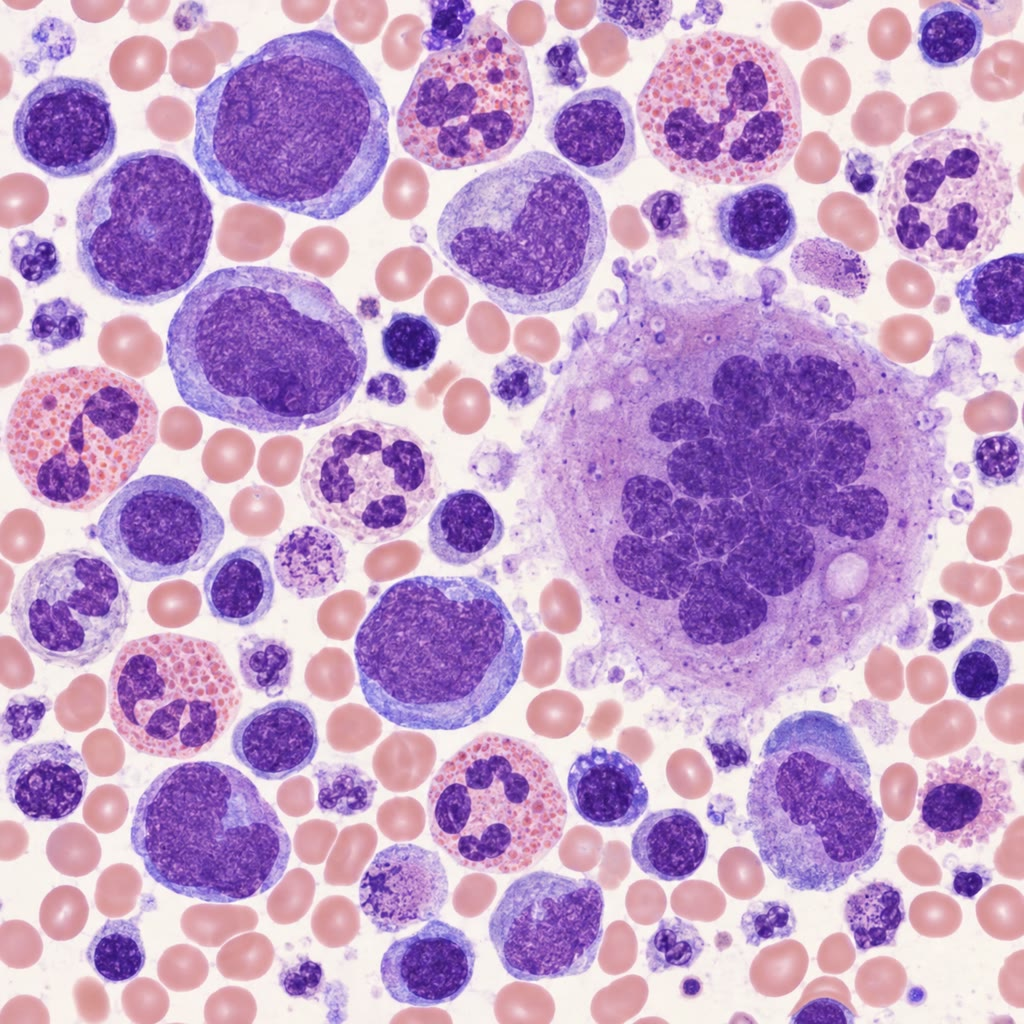
\includegraphics[width=0.4\linewidth]{images/book5/ai/b5-24-bone-marrow-smear.jpg}

{\small बाएँ: मानव सर्वशक्त कोशिकाओं से उगाया कोई प्रमस्तिष्कीय
\omterm{def:b3:stem-cells:pluripotency}{ऑर्गेनॉइड} --- यानी कुछ मिलीमीटर का स्वयं-संगठित प्रांतस्था-सरीखा ऊतक,
जिसमें निलय-सरीखी गुहाएँ और परतदार न्यूरॉन हैं। दाएँ: कोई अस्थि-मज्जा
लेप, जिसमें पहले चित्र की पदानुक्रमी एक साथ दिखती है: विस्फोटकाणु,
परिपक्व होते कणिकाणु, लाल-कोशिका पूर्ववर्ती और कोई महाकेंद्रकाणु।}
\end{omfigure}

\begin{method}[वंशक्रम-अनुरेखण]\label{met:b3:stem-cells:tracing}
\index{वंशक्रम-अनुरेखण}\index{Cre पुनर्संयोजेज़}
यह खोजने के लिए कि किसी ऊतक की \omterm{def:b3:stem-cells:stem}{मूल कोशिकाएँ} कौन-सी हैं: (1) उम्मीदवार
कोशिकाओं द्वारा अभिव्यक्त कोई जीन चुनिए और उसके प्रवर्तक के नीचे कोई
प्रेरणीय पुनर्संयोजेज़ रखिए (Cre-ER, जो केवल टैमॉक्सिफ़ेन दिए जाने पर
सक्रिय होती है); (2) उसी प्राणी में, कोई ऐसा प्रतिवेदक जीन जो तब
स्थायी रूप से सक्रिय हो जाए जब वह पुनर्संयोजेज़ उसमें से कोई विराम-कैसेट
काट दे --- यानी कोई ऐसा रंग जो हर वंशज को विरासत में मिले; (3) उन
उम्मीदवार कोशिकाओं को किसी एक क्षण चिह्नित करने के लिए टैमॉक्सिफ़ेन की
एक मात्रा दीजिए; (4) अंतरालों पर ऊतक निकालिए और चिह्नित क्लोन आँकिए: जो
क्लोन बढ़े, महीनों टिके और उस ऊतक का हर कोशिका-प्रकार रखे वह किसी \omterm{def:b3:stem-cells:stem}{मूल
कोशिका} से आया; और जो क्लोन हफ़्ते भर में झड़ जाए वह किसी संक्रमण-कोशिका
से। (5) किसी बहुरंगी प्रतिवेदक के साथ, क्लोनों के बीच की स्पर्धा का
पीछा कीजिए। (6) उसी प्रवर्तक के नीचे अभिव्यक्त किसी विष-ग्राही से उन
चिह्नित कोशिकाओं को मारकर प्रकार्य सीधे जाँचिए, और देखिए कि क्या वह ऊतक
नवीकरण में विफल होता है।
\end{method}

\section{पुनर्जनन}

\begin{definition}[प्राणी फिर कैसे उगाते हैं]\label{def:b3:stem-cells:regeneration}
\index{पुनर्जनन}\index{नियोब्लास्ट}\index{ब्लास्टीमा}\index{विभेदन-निरसन}\index{प्रतिपूरक वृद्धि}
पुनर्जनन तीन रास्ते लेता है। \emph{Hydra} और प्लेनेरिया वयस्क सर्वशक्त
\omterm{def:b3:stem-cells:stem}{मूल कोशिकाओं} पर टिके हैं: प्लेनेरिया के \emph{नियोब्लास्ट}, जो उसकी
कोशिकाओं का पाँचवाँ भाग हैं, उसकी इकलौती बँटती कोशिकाएँ हैं, जो किसी
घाव तक प्रवास करती हैं और स्थानिक संकेतों के मार्गदर्शन में कोई भी
ग़ायब हिस्सा फिर बना देती हैं (कोई Wnt प्रवणता उस टुकड़े को बताती है कि
कौन-सा सिरा पूँछ है; उसे रोक दीजिए और कोई पूँछ-टुकड़ा दूसरा सिर उगा
लेता है)। सैलामैंडर किसी \emph{ब्लास्टीमा} से कोई उपांग फिर बनाते हैं,
यानी उस ठूँठ पर बँटती कोशिकाओं की किसी ऐसी टोपी से जो बड़े हिस्से में
\emph{विभेदन-निरसन} से बनती है: पेशी-तंतु एककेंद्रकी कोशिकाओं में टूट
जाते हैं, उपास्थि तथा संयोजी कोशिकाएँ किसी \omterm{def:b3:stem-cells:stem}{पूर्वगामी} अवस्था में लौट आती
हैं, और हर एक को अपना उद्गम-ऊतक तथा उस उपांग पर अपनी स्थिति याद रहती है,
और वह ब्लास्टीमा घाव-अधिचर्म तथा उन तंत्रिकाओं के तहत भ्रूणीय
उपांग-कार्यक्रम फिर चला देता है जिनकी उपस्थिति ज़रूरी है (उस ठूँठ की
तंत्रिका काट दीजिए और कुछ नहीं उगता)। ज़ेब्राफ़िश उसी तरह पंख तथा हृदय
फिर उगा लेती है, और उसके हृदय की बची पेशी-कोशिकाएँ बँटकर महीने भर में
उस निलय का पाँचवाँ भाग बदल देती हैं। स्तनी इसमें से बहुत कम करते हैं:
यकृत दो-तिहाई निकाल दिए जाने के बाद अपना द्रव्यमान फिर पा लेता है, पर
बची कोशिकाओं के अपनी जगह बँटने से (\emph{प्रतिपूरक वृद्धि}), न कि खोई
पालियाँ फिर बनाकर; बच्चों में उँगली की नोक फिर उग आती है; और हिरन के
सींग हर साल किसी मूल-कोशिका पर्यास्थिकला से नए उगते हैं। इससे अधिक
क्यों नहीं, यह सौदों का प्रश्न है: स्तनी घाव-अनुक्रिया --- तेज़ स्कंदन,
\omterm{def:b3:innate-immunity:inflammation}{शोथ}, तंतुकोरकी व्रणचिह्न --- संक्रमण तथा रक्त-हानि के सामने किसी घाव को
तेज़ बंद कर देती है, और वह व्रणचिह्न ब्लास्टीमा का रास्ता रोक देता है;
और जो कोशिकाएँ मनमर्ज़ी विभेदन-निरसन करके बँट सकती हैं वही कोशिकाएँ
\omterm{def:b3:cancer-biology:hallmarks}{कर्कट} बन सकती हैं, यानी कोई ऐसा जोखिम जो कोई दीर्घजीवी गरम-रक्ती प्राणी
शायद वहन न कर सके।
\end{definition}

\begin{omfigure}
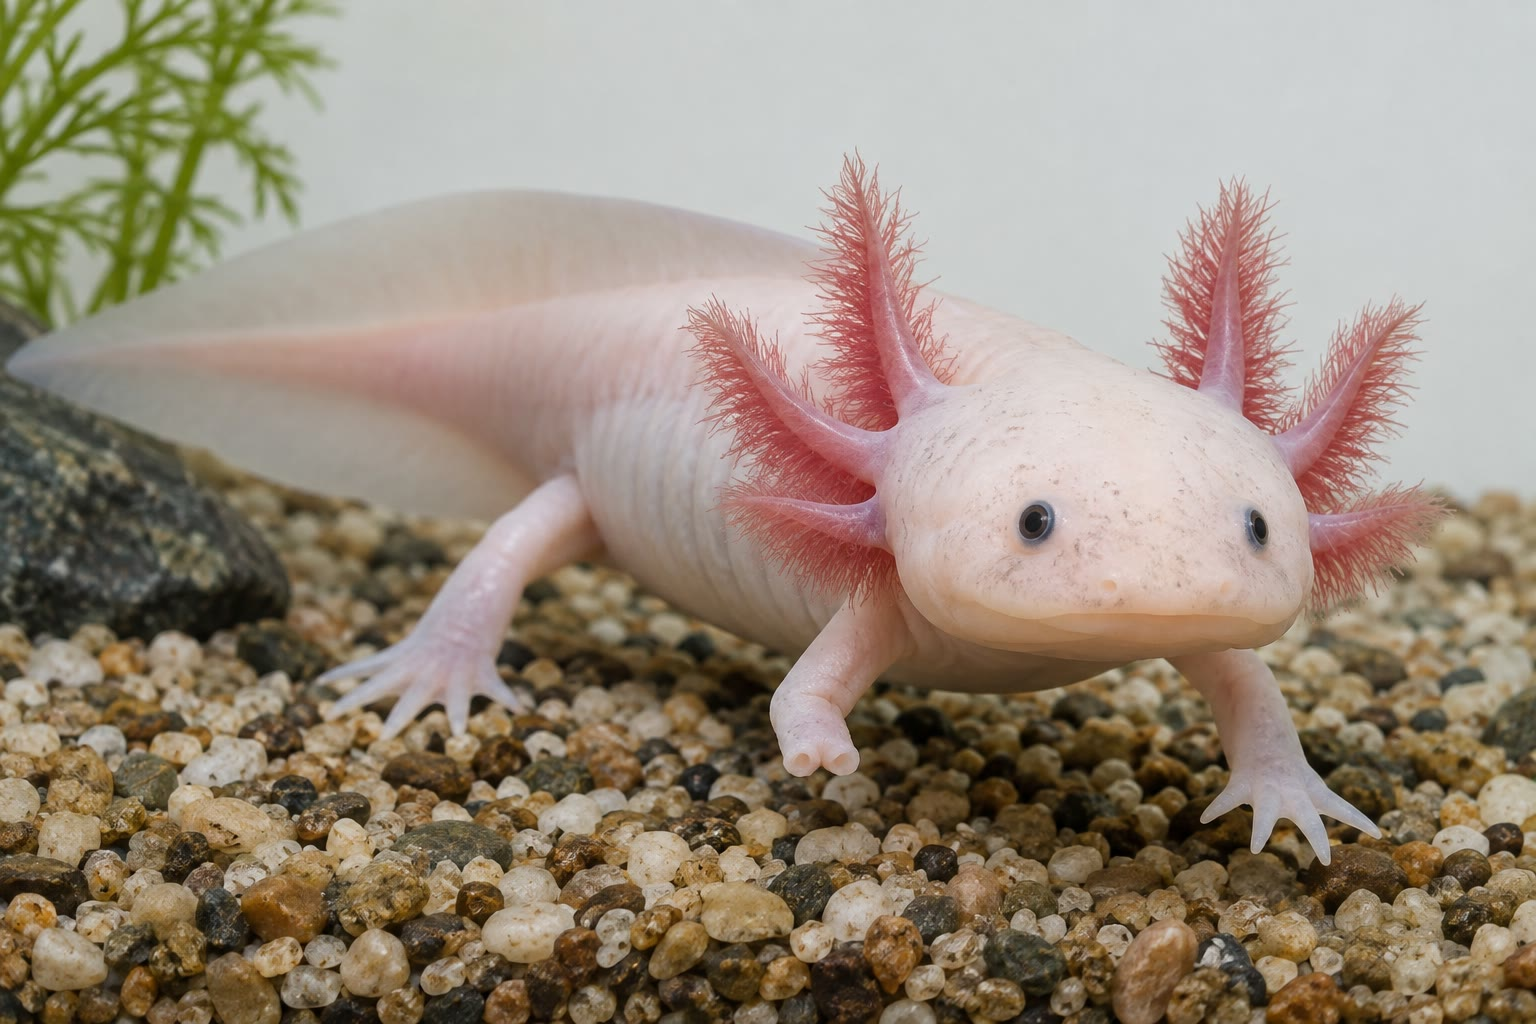
\includegraphics[width=0.46\linewidth]{images/book5/ai/b5-24-axolotl.jpg}\hspace{0.04\linewidth}
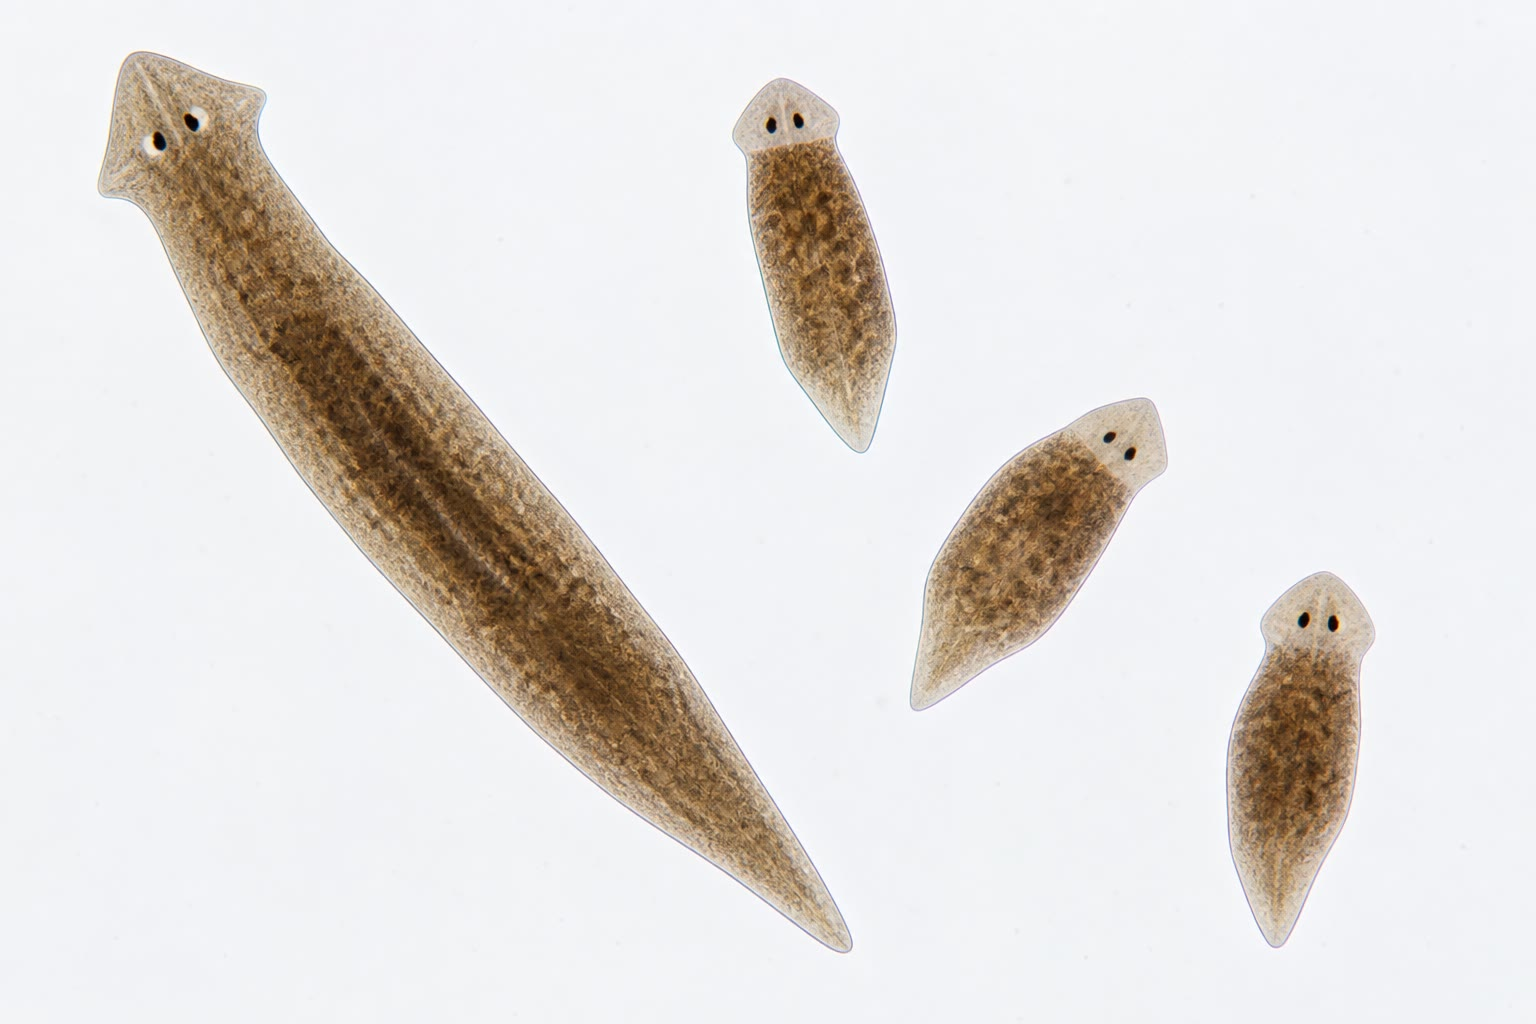
\includegraphics[width=0.46\linewidth]{images/book5/ai/b5-24-planarian-regeneration.jpg}

{\small बाएँ: कोई ऐक्सोलोटल, जो विभेदन-निरसित कोशिकाओं के किसी
\omterm{def:b3:stem-cells:regeneration}{ब्लास्टीमा} से दो महीनों में कोई उपांग फिर उगा लेता है और जीवन भर ऐसा कर
सकता है। दाएँ: टुकड़ों में कटा कोई प्लेनेरिया, जिसका हर टुकड़ा दो
हफ़्तों में अपने \omterm{def:b3:stem-cells:regeneration}{नियोब्लास्टों} से कोई पूरा कृमि फिर उगा लेता है।}
\end{omfigure}

\begin{proof}[प्रमाण-सामग्री]
मॉर्गन (1898) ने प्लेनेरिया को 279 टुकड़ों में काटा और पाया कि हर एक
पूरा कृमि फिर उगा लेता है, और यह उस शरीर के लगभग सौवें भाग की सीमा तक;
रेडियन और सहयोगियों (2011) ने किसी घातक रूप से विकिरणित कृमि में कोई एक
\omterm{def:b3:stem-cells:regeneration}{नियोब्लास्ट} प्रत्यारोपित किया और उसे पूरी तरह लौटा दिया --- यानी एक
कोशिका, हर ऊतक। क्रागल और सहयोगियों (2009) ने ऐसे ऐक्सोलोटल बनाए
जिनके ऊतक एक-एक करके हरे अंकित थे और उन्हें अनंकित परपोषियों में कलमित
किया: विच्छेदन के बाद हरी पेशी ने केवल पेशी दी, हरी उपास्थि ने उपास्थि
--- यानी वह \omterm{def:b3:stem-cells:regeneration}{ब्लास्टीमा} सर्वशक्त कोशिकाओं का कोई पूल नहीं बल्कि
वंश-सीमित \omterm{def:b3:stem-cells:stem}{पूर्वगामियों} का कोई संग्रह है, जिनमें हर एक का \omterm{def:b3:stem-cells:regeneration}{विभेदन-निरसन}
केवल अपने ही ऊतक के \omterm{def:b3:stem-cells:stem}{पूर्वगामी} तक हुआ है। सिंगर (1952) ने दिखाया कि कोई
सैलामैंडर उपांग तभी पुनर्जनित होता है जब तंत्रिका-तंतुओं की कोई देहली
संख्या उस ठूँठ तक पहुँचे, और कि किसी तंत्रिका को पार्श्व के किसी घाव की
ओर मोड़ देने से वहाँ कोई उपांग उग आया।
\end{proof}

\section{वृद्धावस्था का अंकगणित}

\begin{theorem}[टीलोमियर और हेफ़्लिक सीमा]\label{thm:b3:stem-cells:hayflick}
\index{टीलोमियर}\index{हेफ़्लिक सीमा}\index{सिरा-प्रतिकृति समस्या}\index{टीलोमरेज़}\index{प्रतिकृतिक जरण}
हर गुणसूत्र किसी \emph{टीलोमियर} पर समाप्त होता है, यानी पुनरावृत्ति
TTAGGG के कई किलोक्षार पर। चूँकि DNA पॉलीमरेज़ पश्चगामी लड़ी का
आख़िरी हिस्सा पूरा नहीं कर सकती (यानी \emph{\omterm{thm:b3:stem-cells:hayflick}{सिरा-प्रतिकृति समस्या}}), हर
विभाजन हर टीलोमियर को $\Delta \approx$ \qtyrange{50}{100}{bp} छोटा कर
देता है। $L_{0} \approx \qty{10}{kb}$ से शुरू होकर और तब
\emph{\omterm{thm:b3:stem-cells:hayflick}{प्रतिकृतिक जरण}} --- यानी p53 से लागू कोई स्थायी ठहराव --- छेड़ते
हुए, जब सबसे छोटा टीलोमियर $L_{\text{क्रांतिक}} \approx \qty{4}{kb}$ तक
पहुँचे, कोई कोशिका-वंशक्रम अधिक से अधिक
\[
n_{\max} = \frac{L_{0} - L_{\text{क्रांतिक}}}{\Delta} \approx \frac{6000}{50\text{--}100} \approx 60\text{--}120
\]
बार बँट सकता है: यानी \emph{\omterm{thm:b3:stem-cells:hayflick}{हेफ़्लिक सीमा}}, वे पचास-कुछ समष्टि-द्विगुणन
जो मानव तंतुकोरक संवर्ध में रुकने से पहले पूरे करते हैं। एंज़ाइम
\emph{\omterm{def:b3:cancer-biology:telomerase}{टीलोमरेज़}}, यानी कोई RNA-साँचा प्रतिलोम अनुलेखक, उन सिरों को फिर
लंबा कर देती है; वह जनन-वंश में, भ्रूणीय तथा अनेक वयस्क \omterm{def:b3:stem-cells:stem}{मूल कोशिकाओं}
में, और \qty{90}{\%} \omterm{def:b3:cancer-biology:hallmarks}{कर्कटों} में सक्रिय है, जिन्होंने उसे फिर चालू करके
उस सीमा से बच निकलने का रास्ता निकाला। जो \omterm{def:b3:stem-cells:stem}{मूल कोशिका} साल में $d$ बार
बँटती हो और जिसमें \omterm{def:b3:cancer-biology:telomerase}{टीलोमरेज़} उस हानि के किसी अंश $f$ की भरपाई करती हो
उसके पास $n_{\max} = (L_{0} - L_{\text{क्रांतिक}})/[(1 - f)\Delta]$
विभाजन हैं, और $n_{\max}/d$ वर्षों का जीवन: $f = 0.7$, $\Delta
= 60$, $d = 1$ के साथ किसी रुधिरजनक \omterm{def:b3:stem-cells:stem}{मूल कोशिका} के लिए कोई 330 वर्ष ---
पर उसके \omterm{def:b3:stem-cells:stem}{पूर्वगामी}, जिनकी \omterm{def:b3:cancer-biology:telomerase}{टीलोमरेज़} बंद है और जिन्हें किसी लाल कोशिका तक
बीस विभाजन करने हैं, हर वंश-परंपरा पर अपना पाँचवाँ भाग खर्च कर देते हैं,
और इसीलिए बूढ़े लोगों की रक्त-कोशिकाओं के टीलोमियर जवान लोगों से छोटे
होते हैं, प्रति वर्ष लगभग \qty{30}{bp} से।
\end{theorem}
\begin{proof}
प्रति विभाजन हानि कोई नियत लंबाई है, इसलिए टीलोमियर की लंबाई विभाजन-संख्या
के साथ रैखिक रूप से गिरती है, $L_{n} = L_{0} - n\Delta$, और
$L_{\text{क्रांतिक}}$ तक $n = (L_{0} - L_{\text{क्रांतिक}})/\Delta$ पर पहुँचती
है; और आंशिक भरपाई के साथ प्रति विभाजन शुद्ध हानि $(1 - f)\Delta$ है।
हेफ़्लिक और मूरहेड (1961) ने दिखाया कि सामान्य मानव तंतुकोरक, संवर्ध की
परिस्थितियाँ जो भी हों, लगभग पचास द्विगुणनों के बाद रुक जाते हैं, कि
बीस द्विगुणनों के बाद जमाई और फिर पिघलाई गई कोशिकाएँ केवल बचे तीस पूरे
करती हैं --- वे विभाजन गिनती हैं, समय नहीं --- और कि बूढ़े दाताओं की
कोशिकाओं के लिए वह सीमा नीची है। हार्ली, फ़ुचर और ग्राइडर (1990) ने
टीलोमियर को संवर्ध में द्विगुणनों के साथ और दाता की आयु के साथ छोटे होते
नापा; और बॉडनार तथा सहयोगियों (1998) ने सामान्य कोशिकाओं में \omterm{def:b3:cancer-biology:telomerase}{टीलोमरेज़}
डाली और वे उस सीमा के पार अनिश्चित काल तक बँटती रहीं, बिना कर्कटी बने,
और इसी ने उस टीलोमियर को वह घड़ी स्थापित कर दिया।
\end{proof}

\begin{omfigure}
\begin{tikzpicture}
\begin{axis}[
  width=0.62\linewidth, height=5.4cm,
  axis x line=bottom, axis y line=left,
  xmin=0, xmax=120, ymin=0, ymax=11,
  xlabel={समष्टि-द्विगुणन}, ylabel={टीलोमियर की लंबाई (kb)},
  xlabel style={font=\small, at={(axis description cs:0.5,-0.12)}, anchor=north}, ylabel style={font=\small},
  tick label style={font=\small}, xtick={0,30,60,90,120}, ytick={4,7,10},
  clip=false,
]
\addplot[very thick, omDef, domain=0:60, samples=2] {10-0.1*x};
\addplot[very thick, omThm, domain=0:120, samples=2] {10-0.05*x};
\addplot[very thick, omMeth!70!black, domain=0:120, samples=2] {10-0.015*x};
\draw[dashed, gray] (axis cs:0,4) -- (axis cs:120,4); \node[font=\scriptsize, gray, anchor=north west] at (axis cs:2,3.9) {$L_{\text{क्रांतिक}} = \qty{4}{kb}$ पर जरण};
\node[font=\scriptsize, omDef, anchor=south west] at (axis cs:63,4.3) {$\Delta = \qty{100}{bp}$: 60 द्विगुणन};
\node[font=\scriptsize, omThm, anchor=west] at (axis cs:70,8.0) {$\Delta = \qty{50}{bp}$: 120};
\node[font=\scriptsize, omMeth!70!black, anchor=south west, align=left] at (axis cs:78,9.3) {टीलोमरेज़ \qty{70}{\%}\\की भरपाई करती: 400};
\fill[omDef] (axis cs:60,4) circle (2pt); \fill[omThm] (axis cs:120,4) circle (2pt);
\end{axis}
\end{tikzpicture}

{\small विभाजन-गणक के रूप में टीलोमियर। प्रति विभाजन नियत हानि कोई सीधी
रेखा देती है; और जहाँ वह क्रांतिक लंबाई पार करती है वहाँ वह वंशक्रम रुक
जाता है। \omterm{def:b3:cancer-biology:telomerase}{टीलोमरेज़} उस ढाल को चपटा कर देती है और, पूरी तरह सक्रिय हो तो,
उस सीमा को मिटा देती है --- जनन-वंश में, और \omterm{def:b3:cancer-biology:hallmarks}{कर्कटों} में।}
\end{omfigure}

\begin{proposition}[गोंपर्ट्ज़ का नियम]\label{prop:b3:stem-cells:gompertz}
\index{गोंपर्ट्ज़ का नियम}\index{मृत्यु-दर}\index{वृद्धावस्था के लक्षण}\index{जीर्ण कोशिका}
लगभग तीस के ऊपर मानव मृत्यु-दर $\mu(t)$ --- यानी अगले वर्ष में मरने की
प्रायिकता --- हर आठ वर्षों में दुगुनी हो जाती है: $\mu(t) =
\mu_{0}\,\mathrm{e}^{\gamma(t - t_{0})}$, जिसमें $\gamma = \ln 2/8 \approx
\qty{0.087}{yr^{-1}}$ (गोंपर्ट्ज़, 1825)। तब आयु $t$ तक जीवित रहना है
\[
S(t) = \exp\!\Bigl[-\frac{\mu_{0}}{\gamma}\bigl(\mathrm{e}^{\gamma(t - t_{0})} - 1\bigr)\Bigr],
\]
यानी कोई ऐसा वक्र जो दशकों तक चपटा है और फिर तीखा गिरता है, जिसका
मध्यक जीवनकाल $t_{1/2} = t_{0} + \gamma^{-1}\ln(1 + \gamma\ln 2/\mu_{0})$
है: तीस पर प्रति वर्ष $\mu_{0} = 10^{-3}$ के लिए, लगभग $30 + 47 = 77$
वर्ष। वही नियम, भिन्न अचरों के साथ, चूहों (द्विगुणन-काल तीन महीने),
कुत्तों, मक्खियों और कृमियों के लिए भी चलता है: वृद्धावस्था भेद्यता में
कोई चरघातांकी बढ़त है, कोई ठहर जाती घड़ी नहीं। उस घातांक के पीछे का
जीव-विज्ञान अंतःक्रिया करते \emph{लक्षणों} का कोई समुच्चय है: जमा हुई
DNA-क्षति और बहिर्जननिक अपवाह, टीलोमियर का घिसाव, प्रोटीन-समस्थापन का
लोप, सूत्रकणिकीय गिरावट, मूल-कोशिका पूलों का चुकना, उन \emph{जीर्ण
कोशिकाओं} का जमाव जो अब बँटती नहीं पर शोथकारी संकेत स्रवित करती हैं, और
चिरकारी \omterm{def:b3:innate-immunity:inflammation}{शोथ}; चूहों में \omterm{prop:b3:stem-cells:gompertz}{जीर्ण कोशिकाएँ} साफ़ करना या कैलोरी घटाना जीवन
बढ़ा देता है, और कृमियों में इंसुलिन-सरीखे पथ का कोई एक उत्परिवर्तन उसे
दुगुना कर देता है। मनुष्यों में वह घातांक घटाया जा सकता है या नहीं, न कि
वह अचर $\mu_{0}$ जिसे चिकित्सा ने सदी भर में दस गुना घटाया है, यही खुला
प्रश्न है।
\end{proposition}
\begin{proof}
यदि $\mu$ वह संकट हो, तो $\mathrm{d}S/\mathrm{d}t = -\mu(t)S$, इसलिए
$\ln S =
-\int_{t_{0}}^{t}\mu = -(\mu_{0}/\gamma)(\mathrm{e}^{\gamma(t-t_{0})} -
1)$। $S = 1/2$ रखने पर: $\mathrm{e}^{\gamma(t-t_{0})} = 1 + \gamma\ln 2/
\mu_{0}$, जिससे वह मध्यक मिलता है; और $\gamma = 0.087$ तथा $\mu_{0} =
10^{-3}$ के साथ, $\ln(1 + 60) = 4.1$, $t - t_{0} = 47$। वह आनुभविक नियम
गोंपर्ट्ज़ का अंग्रेज़ी जीवन-सारणियों पर फिट है; और यह कि वह इतनी
जातियों का वर्णन किसी साझा रूप तथा जाति-विशिष्ट अचरों से करता है, यहाँ
सदी भर की जनांकिकी के सारांश के रूप में स्वीकार कर लिया गया है।
\end{proof}

\begin{omfigure}
\begin{tikzpicture}
\begin{semilogyaxis}[
  width=0.5\linewidth, height=5.2cm,
  axis x line=bottom, axis y line=left,
  xmin=20, xmax=100, ymin=0.0003, ymax=1,
  xlabel={आयु (वर्ष)}, ylabel={प्रति वर्ष मृत्यु-दर},
  xlabel style={font=\small, at={(axis description cs:0.5,-0.12)}, anchor=north}, ylabel style={font=\small},
  tick label style={font=\small}, xtick={30,50,70,90}, ytick={0.001,0.01,0.1,1}, yticklabels={0.001,0.01,0.1,1},
  clip=false,
]
\addplot[very thick, omDef, domain=30:100, samples=2] {0.001*exp(0.0866*(x-30))};
\node[font=\scriptsize, omDef, anchor=north west, align=left] at (axis cs:32,0.3) {$\mu = \mu_{0}\,\mathrm{e}^{\gamma(t-30)}$\\हर 8 वर्षों में दुगुनी};
\end{semilogyaxis}
\begin{axis}[
  at={(0.55\linewidth,0)}, anchor=south west,
  width=0.43\linewidth, height=5.2cm,
  axis x line=bottom, axis y line=left,
  xmin=20, xmax=110, ymin=0, ymax=1.05,
  xlabel={आयु (वर्ष)}, ylabel={जीवित अंश},
  xlabel style={font=\small, at={(axis description cs:0.5,-0.12)}, anchor=north}, ylabel style={font=\small},
  tick label style={font=\small}, xtick={30,50,77,100}, ytick={0.5,1},
  clip=false,
]
\addplot[very thick, omThm, domain=30:110, samples=80] {exp(-(0.001/0.0866)*(exp(0.0866*(x-30))-1))};
\draw[dashed, gray] (axis cs:77,0) -- (axis cs:77,0.5) -- (axis cs:20,0.5);
\node[font=\scriptsize, omThm, anchor=north east, align=right] at (axis cs:75,0.45) {मध्यक\\77 वर्ष};
\end{axis}
\end{tikzpicture}

{\small \omterm{prop:b3:stem-cells:gompertz}{गोंपर्ट्ज़ का नियम}। बाएँ: किसी लघुगणकीय अक्ष पर मृत्यु-दर तीस से
आगे कोई सीधी रेखा है। दाएँ: उससे निकलता जीवन-वक्र --- कोई पठार, फिर
कोई चट्टान, और मध्यक वहाँ जहाँ उस संकट का समाकल $\ln 2$ तक पहुँचे।}
\end{omfigure}

\begin{remark}[नवीकरण और उसकी कीमत]\label{rem:b3:stem-cells:remark}
जो शरीर अपना नवीकरण करे उसे ऐसी कोशिकाएँ रखनी ही पड़ती हैं जो अनिश्चित
काल तक बँट सकें, और जो कोशिकाएँ अनिश्चित काल तक बँट सकें वही \omterm{def:b3:cancer-biology:hallmarks}{कर्कट} की
सामग्री हैं; और जो शरीर विभाजन गिनकर तथा जरण लागू करके \omterm{def:b3:cancer-biology:hallmarks}{कर्कट} से बचाव
करे उसके पास समय के साथ बँट सकने वाली कोशिकाएँ कम पड़ ही जाएँगी।
मूल-कोशिका पदानुक्रमी एक हल है --- \omterm{def:b3:stem-cells:stem}{कोटरों} में सुरक्षित कुछ धीमी
कोशिकाएँ, और अनेक तेज़ कोशिकाएँ जो जल्दी मर जाती हैं --- और \omterm{thm:b3:stem-cells:hayflick}{हेफ़्लिक
सीमा} दूसरा, और गोंपर्ट्ज़ का चरघातांक उनकी लागतों का योग है। सैलामैंडर
अलग तरह से चुकाता है: वह ऐसी कोशिकाएँ सह लेता है जो \omterm{def:b3:stem-cells:regeneration}{विभेदन-निरसन} करती
हैं और कोई टाँग फिर उगा लेता है, और वह ठंडे-रक्ती, धीमा है और इतना लंबा
शायद ही जीता है कि उसे \omterm{def:b3:cancer-biology:hallmarks}{कर्कट} का बिल चुकाना पड़े। जिन कोशिकाओं के साथ आप
जन्मे थे वे, बड़े हिस्से में, वे नहीं जो आपके पास हैं; और जिन्होंने वे
बदलियाँ बनाईं वही हैं जिन्हें आपको रखना है।
\end{remark}

\section{अभ्यास}

\begin{exercise}[$\star$]\label{exo:b3:stem-cells:1}
\omterm{def:b3:stem-cells:stem}{स्व-नवीकरण}, शक्ति, \omterm{def:b3:stem-cells:stem}{कोटर} और \omterm{def:b3:stem-cells:stem}{संक्रमण-प्रवर्धी कोशिका} परिभाषित कीजिए, और
आँत में हर एक का एक-एक उदाहरण दीजिए।
\end{exercise}

\begin{exercise}[$\star$]\label{exo:b3:stem-cells:2}
प्लीहा-बस्ती परीक्षण ने क्या दिखाया, और किसी \omterm{def:b3:stem-cells:stem}{मूल कोशिका} के किस गुण को
दिखाने के लिए कोई दूसरा चूहा चाहिए था?
\end{exercise}

\begin{exercise}[$\star$]\label{exo:b3:stem-cells:3}
यामानाका के चारों कारक बताइए और समझाइए कि \omterm{def:b3:stem-cells:pluripotency}{पुनःक्रमण} में हफ़्ते क्यों
लगते हैं और वह हज़ारवें भाग कोशिकाओं में ही क्यों सफल होता है।
\end{exercise}

\begin{exercise}[$\star$]\label{exo:b3:stem-cells:4}
प्लेनेरिया और सैलामैंडर के \omterm{def:b3:stem-cells:regeneration}{पुनर्जनन} के रास्तों की तुलना कीजिए, और
बताइए कि क्रागल के कलमन-प्रयोगों ने उस \omterm{def:b3:stem-cells:regeneration}{ब्लास्टीमा} के बारे में क्या
दिखाया।
\end{exercise}

\begin{exercise}[$\star\star$]\label{exo:b3:stem-cells:5}
टीलोमियर \qty{11}{kb} से शुरू होते हैं, जरण \qty{5}{kb} पर, और हानि
प्रति विभाजन \qty{75}{bp}। \omterm{thm:b3:stem-cells:hayflick}{हेफ़्लिक सीमा}? किसी 70 वर्ष के दाता की
कोशिकाओं के पास \qty{8}{kb} हैं: बचे द्विगुणन? यदि \omterm{def:b3:cancer-biology:telomerase}{टीलोमरेज़} उस हानि
के \qty{60}{\%} की भरपाई करे, तो सीमा?
\end{exercise}

\begin{exercise}[$\star\star$]\label{exo:b3:stem-cells:6}
किसी क्रिप्ट में 14 \omterm{def:b3:stem-cells:stem}{मूल कोशिकाएँ} दिन में एक बार बँटती हैं और उन
संक्रमण-कोशिकाओं को खिलाती हैं जो 4 बार और बँटती हैं, और वह क्रिप्ट
अपने रसांकुर को दिन भर में \num{300} कोशिकाएँ जुटाता है। वह अंकगणित
जाँचिए: दिन भर में कितने मूल-कोशिका विभाजन विभेदित होती संततियाँ बनाते
हैं, और वह कितनी \omterm{def:b3:stem-cells:stem}{मूल कोशिकाओं} जितने विभाजन हुए?
\end{exercise}

\begin{exercise}[$\star\star$]\label{exo:b3:stem-cells:7}
वह शरीर दिन भर में $2\times 10^{11}$ लाल कोशिकाएँ बनाता है, जिनमें से
हर एक किसी \omterm{def:b3:stem-cells:stem}{मूल कोशिका} से लगभग 20 विभाजनों का उत्पाद है। इसके लिए दिन
भर में कितने मूल-कोशिका विभाजन चाहिए, और \num{10000} \omterm{def:b3:stem-cells:stem}{मूल कोशिकाओं} के
साथ हर एक कितनी बार बँटती है? देखे गए ``लगभग साल में एक बार'' से तुलना
कीजिए और उस अंतर की व्याख्या कीजिए।
\end{exercise}

\begin{exercise}[$\star\star$]\label{exo:b3:stem-cells:8}
$\gamma = \qty{0.087}{yr^{-1}}$ के साथ और तीस पर $\mu_{0} = 10^{-3}$ के
साथ, 50, 70 और 90 पर मृत्यु-दर, 70 तथा 90 तक जीवित रहना, और मध्यक
जीवनकाल निकालिए। $\mu_{0}$ आधा करने से उस मध्यक का क्या होता है?
$\gamma$ आधा करने से क्या?
\end{exercise}

\begin{exercise}[$\star\star$]\label{exo:b3:stem-cells:9}
किसी चूहे का दो-तिहाई यकृत निकाल दिया जाता है। बची यकृतकोशिकाएँ, जो सब
बँटती हैं, दस दिनों में वह द्रव्यमान लौटा देती हैं। हर एक को कितने
विभाजन चाहिए? इसे \omterm{def:b3:stem-cells:regeneration}{पुनर्जनन} नहीं बल्कि \omterm{def:b3:stem-cells:regeneration}{प्रतिपूरक वृद्धि} क्यों कहते हैं,
और वह यकृत क्या \emph{नहीं} फिर बनाता?
\end{exercise}

\begin{exercise}[$\star\star\star$]\label{exo:b3:stem-cells:10}
\omterm{prop:b3:stem-cells:crypt}{उदासीन अपवाह}: किसी \omterm{def:b3:stem-cells:stem}{कोटर} में $N$ \omterm{def:b3:stem-cells:stem}{मूल कोशिकाएँ} सममित रूप से बँटती हैं; हर
घटना पर कोई एक कोशिका बँटती है और कोई एक यादृच्छिक रूप से खो जाती है,
इसलिए किसी दिए क्लोन की संख्या $0$ और $N$ के बीच कोई यादृच्छिक चलन करती
है। तर्क दीजिए कि $k$ कोशिकाओं के किसी क्लोन के अंततः उस \omterm{def:b3:stem-cells:stem}{कोटर} पर क़ब्ज़ा
कर लेने की प्रायिकता $k/N$ है, और $N = 14$ के साथ किसी एक-कोशिका क्लोन
की संभावना $1/14$ है। किसी नए उदासीन उत्परिवर्तन को ढोती किसी \omterm{def:b3:stem-cells:stem}{मूल कोशिका}
के भवितव्य के लिए इससे क्या पूर्वानुमान निकलता है?
\end{exercise}

\begin{exercise}[$\star\star\star$]\label{exo:b3:stem-cells:11}
किसी उत्परिवर्तन से किसी मूल-कोशिका क्लोन को \cref{exo:b3:stem-cells:10}
की स्पर्धा में \qty{10}{\%} का लाभ मिलता है। गुणात्मक रूप से समझाइए कि
उसके क़ब्ज़े की प्रायिकता $k/N$ से कहीं ऊपर क्यों चढ़ जाती है, बूढ़े
लोगों के क्रिप्ट तथा मज्जा उत्तरोत्तर कुछ ही क्लोनों के क़ब्ज़े में
क्यों आते जाते हैं (क्लोनी रुधिरजनन), और यह \omterm{def:b3:cancer-biology:hallmarks}{कर्कट} हुए बिना \omterm{def:b3:cancer-biology:hallmarks}{कर्कट} की ओर
पहला क़दम क्यों है।
\end{exercise}

\begin{exercise}[$\star\star\star$]\label{exo:b3:stem-cells:12}
मान लीजिए गोंपर्ट्ज़ का घातांक $\gamma$ क्षति जमा होने की किसी दर को
दिखाता है और वह अचर $\mu_{0}$ उस परिवेश को। चिकित्सा ने 1900 से
$\mu_{0}$ दस गुना घटाया है पर $\gamma$ नहीं बदला। उस दस गुनी कमी से
मध्यक जीवनकाल में जो बढ़त मिलती है वह निकालिए, और किसी और दस गुनी कटौती
से मिलती और बढ़त; समझाइए कि वह प्रतिफल क्यों घटता जाता है, और इसके बजाय
$\gamma$ में \qty{20}{\%} की कटौती क्या करती।
\end{exercise}

\section{समस्या: वे कोशिकाएँ जिनके साथ आप जन्मे}

\begin{problem}[{सप्तांत समस्या --- संख्याओं में किसी शरीर का नवीकरण:
रक्त की पदानुक्रमी और वह अपनी मूल कोशिकाओं से क्या माँगती है, क्रिप्ट
का अपवाह, टीलोमियर की घड़ी और टीलोमरेज़ तथा पूर्वगामी उसे कैसे खर्च
करते हैं, उस समष्टि का गोंपर्ट्ज़ वक्र, और वे सौदे जो कोई पुनर्जनन करता
प्राणी स्वीकार करता है, जिसका अंत हेफ़्लिक गिनती पर होता है, मूल कोशिका
के जीवन भर के भंडार पर, और मध्यक जीवनकाल पर}]
\label{pb:b3:stem-cells:1}
आँकड़े: दिन भर में लाल कोशिकाएँ $2.5\times 10^{11}$, कणिकाणु
$10^{11}$; \omterm{def:b3:stem-cells:stem}{मूल कोशिका} से परिपक्व कोशिका तक $20$ विभाजन; \num{10000}
रुधिरजनक \omterm{def:b3:stem-cells:stem}{मूल कोशिकाएँ}। टीलोमियर: $L_{0} = \qty{10}{kb}$,
$L_{\text{क्रांतिक}} = \qty{4}{kb}$, प्रति विभाजन $\Delta = \qty{60}{bp}$;
\omterm{def:b3:stem-cells:stem}{मूल कोशिकाओं} में \omterm{def:b3:cancer-biology:telomerase}{टीलोमरेज़} $f = 0.7$ की भरपाई करती है; \omterm{def:b3:stem-cells:stem}{पूर्वगामियों} में
कोई नहीं। क्रिप्ट: $N = 14$ \omterm{def:b3:stem-cells:stem}{मूल कोशिकाएँ}, दिन में एक विभाजन।
गोंपर्ट्ज़: आयु 30 पर प्रति वर्ष $\mu_{0} =
10^{-3}$, $\gamma = \qty{0.087}{yr^{-1}}$। ऐक्सोलोटल का उपांग:
\qty{60}{d} में \qty{40}{mm} फिर उगा; \omterm{def:b3:stem-cells:regeneration}{ब्लास्टीमा} $10^{5}$ कोशिकाओं से
बढ़कर $10^{8}$।

\medskip
\noindent\textbf{भाग I --- रक्त।}
\begin{enumerate}
  \item दिन भर में कुल बनी कोशिकाएँ, और प्रति सेकंड।
  \item हर परिपक्व कोशिका $20$ विभाजनों का अंत है: किसी \omterm{def:b3:stem-cells:stem}{मूल कोशिका} की
        किसी एक प्रतिबद्ध संतति से कितनी कोशिकाएँ निकलती हैं? दिन भर
        में कितनी प्रतिबद्ध संततियाँ चाहिए?
  \item \num{10000} \omterm{def:b3:stem-cells:stem}{मूल कोशिकाओं} के साथ, इससे प्रति \omterm{def:b3:stem-cells:stem}{मूल कोशिका} प्रति
        दिन कितने विभेदन-विभाजन निकलते हैं? प्रति वर्ष?
  \item नापा गया मूल-कोशिका विभाजन लगभग साल में एक बार है। मेल बिठाइए:
        उन \omterm{def:b3:stem-cells:stem}{पूर्वगामियों} को वह क्या करना चाहिए जो प्रश्न~3 की गणना ने
        मान लिया था कि \omterm{def:b3:stem-cells:stem}{मूल कोशिकाएँ} करती हैं?
  \item \omterm{def:b3:stem-cells:stem}{पूर्वगामियों} में कोई \omterm{def:b3:cancer-biology:telomerase}{टीलोमरेज़} नहीं। \qty{10}{kb} से, किसी
        लाल-कोशिका पूर्ववर्ती के टीलोमियर अपने $20$ विभाजनों के बाद
        कौन-सी लंबाई तक पहुँचते हैं? क्या यह मायने रखता है कि वह
        $L_{\text{क्रांतिक}}$ से ऊपर है?
  \item $f = 0.7$ के साथ साल में एक बार बँटती कोई \omterm{def:b3:stem-cells:stem}{मूल कोशिका}: प्रति
        विभाजन शुद्ध हानि, जरण तक विभाजन, और वर्ष। टिप्पणी कीजिए।
\end{enumerate}

\medskip
\noindent\textbf{भाग II --- क्रिप्ट।}
\begin{enumerate}[resume]
  \item मूल-कोशिका तह पर प्रति क्रिप्ट प्रति दिन विभाजन; यदि आधी
        घटनाएँ किसी खोई \omterm{def:b3:stem-cells:stem}{मूल कोशिका} की जगह भरें और आधी उस
        संक्रमण-क्षेत्र को खिलाएँ, तो दिन भर में कितनी प्रतिबद्ध
        कोशिकाएँ, और $4$ संक्रमण-विभाजनों के बाद कितनी रसांकुर-कोशिकाएँ?
  \item किसी एक-कोशिका क्लोन के क़ब्ज़े की प्रायिकता $1/N$ है। एकक्लोनता
        तक का प्रत्याशित समय प्रति कोशिका $N^{2}$ विभाजन-घटनाओं की कोटि
        का है; उसे दिनों में आँकिए और कन्फ़ेटी प्रेक्षणों (महीने) से
        तुलना कीजिए।
  \item किसी \omterm{def:b3:stem-cells:stem}{मूल कोशिका} को कोई उत्परिवर्तन मिलता है। उसके अपने क्रिप्ट
        में अंततः स्थिर हो जाने की प्रायिकता? किसी बृहदांत्र के
        $10^{7}$ क्रिप्टों में से कितनों में, प्रति क्रिप्ट एक बार उठता
        कोई उत्परिवर्तन, स्थिर हो जाता?
  \item किसी ऐसे ऊतक के मुक़ाबले, जिसमें हर \omterm{def:b3:stem-cells:stem}{मूल कोशिका} जीवन भर असममित
        रूप से बँटती हो, किसी क्रिप्ट का अपवाह \omterm{def:b3:cancer-biology:hallmarks}{कर्कट} से अधिक रक्षा
        क्यों करता है?
  \item विकिरण से \omterm{def:b3:stem-cells:stem}{मूल कोशिकाएँ} मर जाने के बाद संक्रमण-कोशिकाएँ पलटकर वह
        \omterm{def:b3:stem-cells:stem}{कोटर} फिर भर देती हैं। इससे इस बारे में क्या पता चलता है कि
        मूलत्व रहता कहाँ है?
  \item वह वंशक्रम-अनुरेखण प्रयोग रेखांकित कीजिए जो सममित अपवाह को
        \omterm{def:b3:stem-cells:stem}{असममित विभाजन} से अलग बताता है, और उसके दोनों परिणाम।
\end{enumerate}

\medskip
\noindent\textbf{भाग III --- वह घड़ी।}
\begin{enumerate}[resume]
  \item बिना \omterm{def:b3:cancer-biology:telomerase}{टीलोमरेज़} के किसी कायिक वंशक्रम के लिए \omterm{thm:b3:stem-cells:hayflick}{हेफ़्लिक सीमा}।
  \item किसी तंतुकोरक संवर्ध को $25$ द्विगुणनों के बाद जमा दिया जाता है
        और दशक भर बाद पिघलाया जाता है: बचे द्विगुणन? इससे इस बारे में
        क्या पता चलता है कि वह कोशिका क्या गिनती है?
  \item वयस्कों में श्वेताणु टीलोमियर प्रति वर्ष \qty{30}{bp} छोटे होते
        हैं। बीस पर \qty{8}{kb} से शुरू होकर, वे $L_{\text{क्रांतिक}}$ तक
        कब पहुँचते? जीवनकाल से तुलना कीजिए और टिप्पणी कीजिए।
  \item सामान्य तंतुकोरकों में डाली गई \omterm{def:b3:cancer-biology:telomerase}{टीलोमरेज़} उन्हें बिना कर्कटी बने
        उस सीमा के पार जाने देती है। \omterm{def:b3:cancer-biology:telomerase}{टीलोमरेज़} \qty{90}{\%} \omterm{def:b3:cancer-biology:hallmarks}{कर्कटों} में
        सक्रिय है। इन दोनों कथनों में मेल बिठाइए।
  \item 40, 60, 80 और 100 पर गोंपर्ट्ज़ मृत्यु-दर, और हर एक तक जीवित
        रहना, निकालिए।
  \item मध्यक जीवनकाल; और वह आयु जिस पर \qty{10}{\%} जीवित रहते हैं।
\end{enumerate}

\medskip
\noindent\textbf{भाग IV --- फिर उगाना।}
\begin{enumerate}[resume]
  \item ऐक्सोलोटल: mm/दिन में माध्य पुनर्वृद्धि-दर; उस \omterm{def:b3:stem-cells:regeneration}{ब्लास्टीमा} को
        $10^{5}$ से $10^{8}$ कोशिकाओं तक बढ़ने के लिए द्विगुणन, और 60
        दिनों भर का माध्य द्विगुणन-काल।
  \item यदि विभेदन-निरसित कोशिकाएँ जीवन भर उस \omterm{def:b3:stem-cells:regeneration}{ब्लास्टीमा} जैसी बँटती हों
        और हर विभाजन प्रति कोशिका किसी अर्बुदजनक उत्परिवर्तन की
        $10^{-9}$ संभावना ढोए, तो किसी एक \omterm{def:b3:stem-cells:regeneration}{पुनर्जनन} में ऐसे कितने
        उत्परिवर्तन उठते हैं? फिर भी वह ऐक्सोलोटल लगभग कभी कर्कटी क्यों
        नहीं होता, और कोई स्तनी इससे बच क्यों न पाता?
  \item उस ठूँठ की तंत्रिका काट देने से \omterm{def:b3:stem-cells:regeneration}{पुनर्जनन} रुक जाता है। यह दिखाने
        के लिए कोई प्रयोग सुझाइए कि वह तंत्रिका कोई विसरणशील कारक
        जुटाती है, और उस कारक की एक संभावित पहचान।
  \item किसी Wnt निरोधक को घटा देने पर प्लेनेरिया का कोई पूँछ-टुकड़ा
        सिर के बजाय दूसरी पूँछ उगा लेता है। किसी प्रवणता और उस टुकड़े की
        स्थानिक स्मृति से समझाइए।
  \item दो-तिहाई उच्छेदन के बाद मानव यकृत: वह द्रव्यमान लौटाने के लिए
        यकृतकोशिकाओं का कितना अंश एक बार, कितना दो बार बँटे। परिणाम कोई
        काम करता यकृत पर ग़लत आकार का क्यों है?
  \item जो शरीर ऐक्सोलोटल की तरह \omterm{def:b3:stem-cells:regeneration}{पुनर्जनन} करता उसका गोंपर्ट्ज़ वक्र
        भिन्न क्यों होता, और किस दिशा में?
  \item सारांश दीजिए: हेफ़्लिक गिनती (प्रश्न~13), किसी टीलोमरेज़-सहित
        \omterm{def:b3:stem-cells:stem}{मूल कोशिका} के विभाजन तथा वर्ष (प्रश्न~6), और मध्यक जीवनकाल
        (प्रश्न~18)।
\end{enumerate}
\end{problem}
